%=======================================================================
% The main source file
%=======================================================================
\documentclass[12pt,a4paper,twoside]{article}

%===== packages =====
\usepackage[dvips]{graphicx}
\usepackage{pst-all}
\usepackage{pst-circ}
\usepackage{listings}

% ===== Paper layout control =====
\setlength  {\voffset}          {0mm}
\setlength  {\hoffset}          {0mm}
\setlength  {\topmargin}        {0mm}
\setlength  {\headheight}       {0mm}
\setlength  {\headsep}          {2mm}
\setlength  {\textwidth}        {140mm}
\setlength  {\textheight}       {220mm}
\setlength  {\marginparwidth}   {30mm}
\setlength  {\marginparsep}     {3mm}
\setlength  {\oddsidemargin}    {10mm}
\setlength  {\evensidemargin}   {10mm}
\setlength  {\parskip}          {2mm}
\setlength  {\parindent}        {0mm}

\addtolength{\headheight}{12pt}

%=== document info ===
\begin{document}

\title{Sample Doc: A minimal example for creating HTML from LaTeX}

\author{Ganga N. N\"adiya}

\thispagestyle{empty}
\maketitle

\setcounter{tocdepth}{1}
\tableofcontents

%=== Section 1 ===
\section{What is this}
Lorem ipsum dolor sit amet, consectetur adipiscing elit. Donec a diam
lectus. Sed sit amet ipsum mauris. Maecenas congue ligula ac quam
viverra nec consectetur ante hendrerit. Donec et mollis dolor. Praesent
et diam eget libero egestas mattis sit amet vitae augue. Nam tincidunt
congue enim, ut porta lorem lacinia consectetur. Donec ut libero sed
arcu vehicula ultricies a non tortor. 

%=== Section 2 ===
\section{Pictures and diagrams}

\subsection{Including PNG}
%---------------------------
Lorem ipsum dolor sit amet, consectetur adipiscing elit. Donec a diam
lectus. Sed sit amet ipsum mauris. Maecenas congue ligula ac quam
viverra nec consectetur ante hendrerit. Donec et mollis dolor. Praesent
et diam eget libero egestas mattis sit amet vitae augue. Nam tincidunt
congue enim, ut porta lorem lacinia consectetur. Donec ut libero sed
arcu vehicula ultricies a non tortor. 

\begin{figure}[htb]
  \begin{center}
    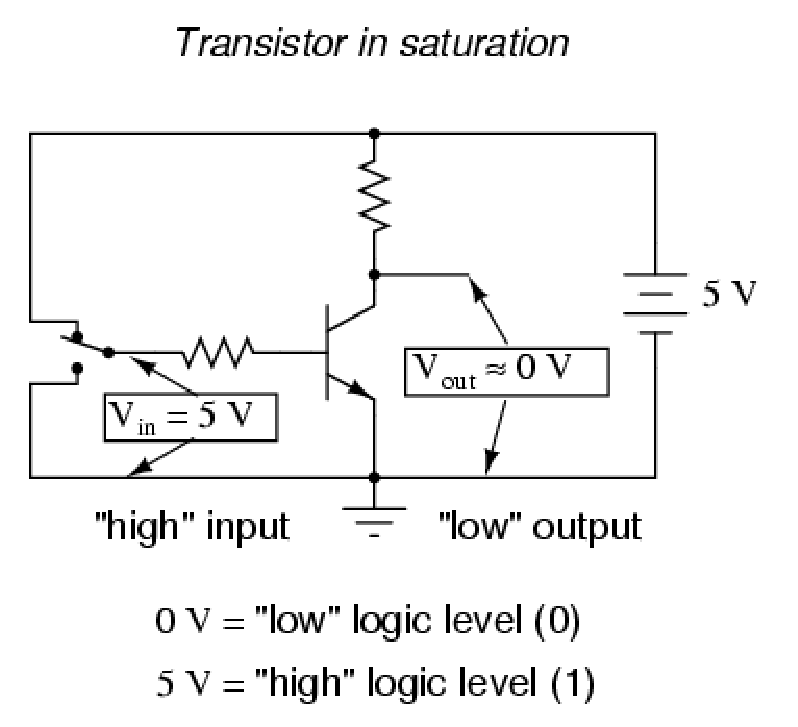
\includegraphics[width=80mm]{images/04068}
    \caption{A PNG included}
  \end{center}
\end{figure}


\subsection{The picture environment}

Vivamus fermentum semper porta. Nunc diam velit, adipiscing ut tristique
vitae, sagittis vel odio. Maecenas convallis ullamcorper ultricies.
Curabitur ornare, ligula semper consectetur sagittis, nisi diam iaculis
velit, id fringilla sem nunc vel mi. Nam dictum, odio nec pretium
volutpat, arcu ante placerat erat, non tristique elit urna et turpis.
Quisque mi metus, ornare sit amet fermentum et, tincidunt et orci. Fusce
eget orci a orci congue vestibulum. Ut dolor diam, elementum et
vestibulum eu, porttitor vel elit. 

\begin{figure}[htb]
  \begin{center}
\setlength{\unitlength}{1cm}
\begin{picture}(4,2)
 \put(0,0){\line(1,0){4}}
 \put(4,0){\line(0,1){2}}
 \put(0,0){\line(2,1){4}}
\end{picture}
    \caption{Picture environment}
  \end{center}
\end{figure}

Nam dictum, odio nec pretium
volutpat, arcu ante placerat erat, non tristique elit urna et turpis.
Quisque mi metus, ornare sit amet fermentum et, tincidunt et orci. Fusce
eget orci a orci congue vestibulum. Ut dolor diam, elementum et
vestibulum eu, porttitor vel elit. 

\subsection{PSTricks}

Vivamus fermentum semper porta. Nunc diam velit, adipiscing ut tristique
vitae, sagittis vel odio. Maecenas convallis ullamcorper ultricies.
Curabitur ornare, ligula semper consectetur sagittis, nisi diam iaculis
velit, id fringilla sem nunc vel mi. Nam dictum, odio nec pretium
volutpat, arcu ante placerat erat, non tristique elit urna et turpis.
Quisque mi metus, ornare sit amet fermentum et, tincidunt et orci. 

\PSTtoEPS[bbllx=-.2,bblly=-0.2,bburx=5,bbury=3]{gus.eps}{%
    \begin{pspicture}(-0.5,-0.5)(5,3)
      \psgrid[subgriddiv=1,griddots=10,gridlabels=7pt](0,0)(4,2)
      \psline[linewidth=2pt]{-}(0,0)(2,2)(4,0)
    \end{pspicture}
}

\begin{figure}[htb]
  \begin{center}
    \includegraphics{gus.eps}
    \caption{PSTricks diagram}
  \end{center}
\end{figure}


%=== Section 3 ===
\section{Source code}
\subsection{C/C++}

Vivamus fermentum semper porta. Nunc diam velit, adipiscing ut tristique
vitae, sagittis vel odio. Maecenas convallis ullamcorper ultricies.
Curabitur ornare, ligula semper consectetur sagittis, nisi diam iaculis
velit, id fringilla sem nunc vel mi. Nam dictum, odio nec pretium
volutpat, arcu ante placerat erat, non tristique elit urna et turpis.
Quisque mi metus, ornare sit amet fermentum et, tincidunt et orci. 
\lstinputlisting{helloworld.c}

\subsection{Matlab}

Vivamus fermentum semper porta. Nunc diam velit, adipiscing ut tristique
vitae, sagittis vel odio. Maecenas convallis ullamcorper ultricies.
Curabitur ornare, ligula semper consectetur sagittis, nisi diam iaculis
velit, id fringilla sem nunc vel mi. Nam dictum, odio nec pretium
volutpat, arcu ante placerat erat, non tristique elit urna et turpis.
Quisque mi metus, ornare sit amet fermentum et, tincidunt et orci. 
\lstinputlisting{cosine.m}

\subsection{Python}

Vivamus fermentum semper porta. Nunc diam velit, adipiscing ut tristique
vitae, sagittis vel odio. Maecenas convallis ullamcorper ultricies.
Curabitur ornare, ligula semper consectetur sagittis, nisi diam iaculis
velit, id fringilla sem nunc vel mi. Nam dictum, odio nec pretium
volutpat, arcu ante placerat erat, non tristique elit urna et turpis.
Quisque mi metus, ornare sit amet fermentum et, tincidunt et orci. 

\begin{lstlisting}[frame=single]
#!/usr/bin/python

# Hello world python program
print "Hello World!";
\end{lstlisting}


%=== Section 4 ===
\section{Math and other symbols}

$$ \lim_{x \to \infty} \exp(-x) = 0 $$

%=== Section 5 ===
\section{Tables}

\begin{center}
  \begin{tabular}{ l | c || r }
    \hline
    1 & 2 & 3 \\ \hline
    4 & 5 & 6 \\ \hline
    7 & 8 & 9 \\
    \hline
  \end{tabular}
\end{center}

\begin{tabular}{|r|l|}
  \hline
  7C0 & hexadecimal \\
  3700 & octal \\ \cline{2-2}
  11111000000 & binary \\
  \hline \hline
  1984 & decimal \\
  \hline
\end{tabular}
\end{document}
